% 	TEMPLATE DE RELACIÓN DE EJERCICIOS
%
% Creador: Juamagdev

% ------------------------------------------------------------------
% ---------------------- Package imports ---------------------------
% ------------------------------------------------------------------
\documentclass[11pt, a4paper]{exam}
\usepackage[utf8]{inputenc}		% UTF-8
\usepackage[spanish]{babel}		% Idioma
\usepackage{graphicx}			% Para importar gráficos
\usepackage{amsthm, amsfonts, amssymb, amssymb} % Todos los paquetes AMS
\usepackage{mathtools}          % Arregla bugs de AMS
\usepackage{hyperref}			% Para \href{URL}{text}
\usepackage{enumitem}			% Para enumerar
\usepackage{color} 				% Para definir colores nuevos
\usepackage{lastpage}			% Para \pageref{LastPage}
\usepackage{booktabs}					% Tablas profesionales
\usepackage{parskip}					% Espacio de párrafos
\usepackage[sharp]{easylist}			% Para litas
\usepackage[expansion=false]{microtype} % Soluciona bugs de tipografias
\usepackage[margin=2.25cm, includehead, includefoot]{geometry}
\usepackage{cancel}
\usepackage{pgfplots}
\usepackage{listings}



% ------------------------------------------------------------------
% ---------------------- Constantes --------------------------------
% ------------------------------------------------------------------
% Las constantes mas importantes
\newcommand{\mytitle}{Ejercicio Máquina de Turing M4}
\newcommand{\mysubject}{Algoritmia y Complejidad}
\newcommand{\mydate}{\today}
\newcommand{\myauthor}{Grupo 04}

% Redefinir para cada caso
\newcommand{\myrhead}{Universidad de Málaga}
\newcommand{\mypagename}{Página}
\newcommand{\mycreated}{Creado por: }
\newcommand{\mysolname}{Solución}
\renewcommand{\solutiontitle}{\noindent\textbf{\mysolname.}\hspace{0.75em}}
\pointpoints{point}{points}

\providecommand{\abs}[1]{\lvert#1\rvert}

% ------------------------------------------------------------------
% ---------------------- Ajustes -----------------------------------
% ------------------------------------------------------------------
% \shadedsolutions
\printanswers % Alternative: \noprintanswers, \printanswers
%\rhead{{\scshape {\footnotesize  \myrhead}}}
%\cfoot{\mypagename \enspace \thepage}
\definecolor{SolutionColor}{rgb}{0.8,0.9,1} % light blue

% Cabeceras y pie de página
\runningfootrule
\firstpagefootrule
\firstpagefooter{\mysubject}{}{\mypagename\ \thepage\ de \pageref*{LastPage}}
\runningfooter{\mysubject}{}{\mypagename\ \thepage\ de \pageref*{LastPage}}
\runningheader{}{}{
\includegraphics[width = 3 cm]{figs/logo.pdf}}
\firstpageheadrule
\firstpageheader{\mydate}{\mytitle}{\pageref*{LastPage} páginas en total}

% Answer command for double lines
\def\answer#1{\underline{\underline{#1}}}

% ------------------------------------------------------------------
% ---------------------- Documento ---------------------------------
% ------------------------------------------------------------------
\begin{document}
\pagestyle{headandfoot}
\noindent {\scshape \Large  \mytitle
    \ifprintanswers
        \enspace (\mysolname	 )
    \fi
} \\
\noindent {\mycreated \enspace  \myauthor} \vspace{1em}
\hrule \hrule
\vspace{5mm}

% ------------------------------------------------------------------
% ---------------------- Contenido ---------------------------------
% ------------------------------------------------------------------

\begin{questions}
    \addpoints
    \question {\bfseries Crea las maquinas de turing para el siguiente lenguaje en su versión multicinta y unicinta:}
    \begin{equation*}
        L = \left\lbrace \#x_1\#x_2\#...\#x_l | x_i \in \left\lbrace 0, 1 \right\rbrace^*, x_i \neq x_j, i\neq j \right\rbrace
    \end{equation*}
    
    \begin{parts}
        \part Multicinta
        \begin{solution}
            \\
            % Una máquina de Turing multicinta es una variante de la máquina de Turing. Es un modelo matemático abstracto de un dispositivo que puede realizar cómputos. A diferencia de la máquina de Turing clásica, que tiene una sola cinta de entrada/salida, la máquina de Turing multicinta tiene varias cintas. En cada cinta, se puede leer y escribir información de entrada y salida.
            El lenguaje que nuestra máquina de Turing que debe reconocer es el de un conjunto finito de palabras formadas por 0s o por 1s, separadas por el símbolo $\#$, con la característica de que no se puede repetir ninguna palabra entre cada $\#$. Es el llamado problema de los elementos distintos.
            \\
            \\
            Es decir, cadenas formadas por 0s y 1s, separadas por $\#$, siempre que no se repitan estas cadenas. Por ejemplo:
            \begin{enumerate}
                \item La cadena $\#100\#11\#101\#00$ es válida.
                \item La cadena $\#000\#10\#111\#000$ no es válida.
                \item La cadena $\#010\#10\#10\#00$ no es válida.
                \item La cadena $\#010\#1011\#01\#0$ es válida.
                \item La cadena $\#\#1\#0$ es válida (la cadena vacía se encuentra una vez)
                \item La cadena $\#\#1\#0\#$ no es válida (la cadena vacía se encuentra dos veces)
            \end{enumerate}
            La máquina de Turing se define sobre los alfabetos:
            \begin{equation*}
                \Gamma = \left\lbrace \#,0,1, \_ \right\rbrace
            \end{equation*}
            \begin{equation*}
                \Sigma = \left\lbrace \#,0,1 \right\rbrace
            \end{equation*}
            que son los mismos, ya que en esta versión multicinta no es necesario añadir símbolos extras.
            \\
            \\
            La máquina de Turing tendrá 2 cintas, en la primera de ellas se pondrá la cadena para ser reconocida, en la segunda es donde se comprobará que no hay cadenas, escribiendo la primera cadena y comparando uno a uno cada elemento. Para ello la má
            quina realiza los siguientes pasos:
            \begin{enumerate}
                \item La máquina copia el separador $\#$ en la segunda cinta y la primera palabra, y los elimina de la primera cinta. Este separador para alinear cada separador y poder comparar dígito por dígito.
                \item Ahora la máquina alinea los separadores de ambas cintas.
                \item A continuación la máquina comprueba símbolo por símbolo que no se repiten. En caso de que encuentre un símbolo que sea distinto, ya no es necesario que compruebe y se dirige al proximo separador. Si todos los símbolos son iguales y no encuentra uno distinto, al llegar al separador rechaza la cadena.
                \item Se ejecutan las pasos 2 y 3 hasta llegar al final (un espacio en blanco).
                \item Al llegar al final, se vuelve al principio y se ejecutan la secuencia de nuevo desde el paso 1.
            \end{enumerate}
            En caso de que la máquina rechace la cadena, se parará mostrando de forma alineada el primer elemento que ha encontrado repetido.
            \\
            \\
            La máquina aceptará la cadena cuando en la primera cinta no haya símbolos. En cualquier otro caso, la cadena sera rechazada.
            A continuación se muestra el autómata que define la máquina de Turing. 
            \\
            \\
            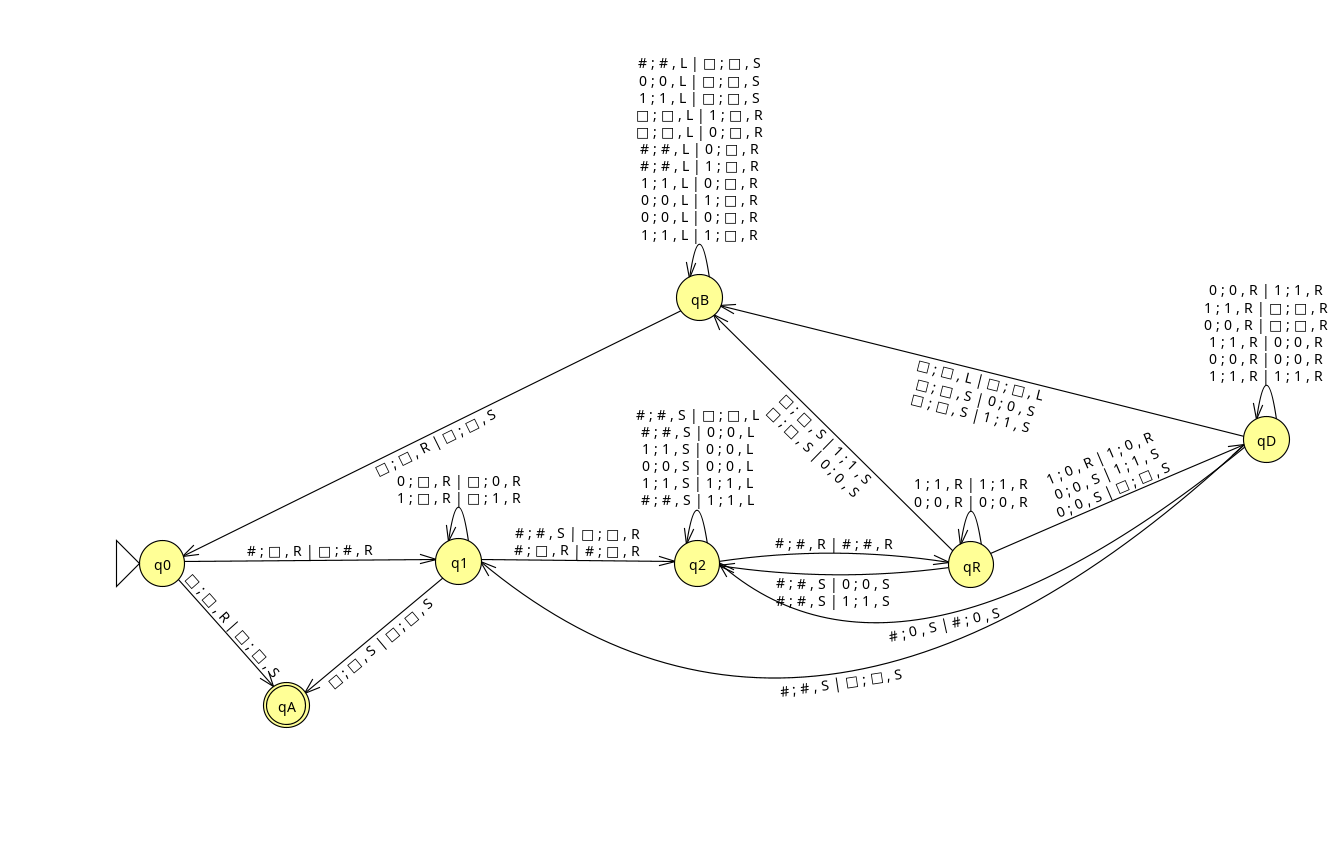
\includegraphics[width = 16 cm]{figs/M4Multicinta.png}
            \\Puede probar la máquina de Turing en el siguiente simulador, donde ya se encuentra cargada la máquina de Turing: \url{http://turingmachinesimulator.com/shared/atughrsuvx}
            \\
            \\
            En cuanto a la complejidad de la máquina, se puede ver que esta tiene dos bucles anidados, por tanto, su complejidad es $O(n^2)$, donde $n$ es el número de símbolos de la cadena.
            \\
            \\
            También puede encontrar todo el código de la máquina usada en el simulador, con los estados y transiciones en el repositorio de \textit{Github}, junto con el autómata generado por JFLAP, dentro de la carpeta de \textit{utilities}:
            \url{https://github.com/juanmagdev/AyC-Grupo-A1-04}
            \\
            \\
            Se puede encontrar la presentación de esta máquina, la cual fue expuesta en clase,  
            \href{https://docs.google.com/presentation/d/1ZGBfp_iIh9p28WokAD8IalFsRS-j9Oyw/edit?usp=sharing&ouid=115190935631983820007&rtpof=true&sd=true}{\color{blue}{este enlace}}.
            \\
            \\
        \end{solution}
        
        \part Unicinta

        \begin{solution}
            \\
            La variante unicinta trabaja sobre la propia cadena que queremos analizar. Para ello debemos asegurarnos de los mismos aspectos que en la máquina multicinta, es decir:
            \begin{enumerate}
                \item Está conformada por subcadenas de 0s y 1s precedidas de $\#$, por tanto la cadena $\#010\#1011\#01\#0$ es válida.
                \item Las subcadenas son distintas dos a dos: La cadena $\#000\#10\#111\#000$ no es válida.
                \item Una subcadena vacía debe ser incluida como válida, pues $\varepsilon \in \left\lbrace 0, 1 \right\rbrace^*$, siempre que no esté repetida: $\#0101\#$ es válida, pero $\#0101\#\#011\#$ no lo es.
            \end{enumerate}
            Para ello, la máquina unicinta deberá tener un lenguaje cinta diferente al lenguaje de entrada, como se explica a continuación.
            \begin{equation*}
                \Gamma = \left\lbrace \#,0,1,o,i,\&,\$,U,\_ \right\rbrace
            \end{equation*}
            \begin{equation*}
                \Sigma = \left\lbrace \#,0,1 \right\rbrace
            \end{equation*}
            \\
            Esta máquina requiere de numerosos estados para poder analizar las cadenas y así reconocerlas o rechazarlas. Se pueden resumir en los pasos siguientes:
            \begin{enumerate}
                \item Comprobamos que no se ha proporcionado la cadena vacía, pues esta debe ser rechazada.
                \item Un puntero de tipo $\&$ reemplaza al $\#$ en una primera subcadena y un segundo puntero de tipo $\$$ al inicio de la segunda, en caso de existir. Estos nos servirán para poder desplazarnos a lo largo de la cinta y comparar cada una de las subcadenas $x_i$ con las que tiene a continuación, $x_j, j>i$. Si hay una única subcadena, entonces hemos acabado (la acepta). Si no, vamos al siguiente paso.
                \item Comparamos cada caracter de manera individual entre las dos cadenas. Para ello, tras la lectura de cada caracter, reemplazamos cada $1$ por $i$ y cada $0$ por $o$. Así la máquina de Turing puede diferenciar qué parte ha sido leída y cual no, sin pérdida de información. Mientras las dos subcadenas sean iguales, seguirá leyendo hasta que encuentre discrepancias, en tal caso pasa al paso siguiente. Si son iguales, rechazará la cadena y habremos terminado.
                \item Al encontrar diferencias entre las subcadenas, dejamos de leerlas y reseteamos el proceso. Para ello, los caracteres $i,o$ vuelven a ser $1,0$. El puntero $\$$ de la segunda cadena pasa a ser un puntero usado, que marcaremos como $U$, para poder diferenciarlo de los demás. A continuación marcaremos la siguiente subcadena sin leer (que empieza por $\#$) con su puntero correspondiente $\$$. Repetimos el proceso desde el paso 2 hasta agotar todas las subcadenas o encontrar dos iguales.
                \item Cuando hemos comparado la primera subcadena (que empieza con $\&$) con todas las posteriores, o lo que es lo mismo, nos topamos con la primera celda vacía \_, entonces debemos hacer un reset de toda la cinta. Los caracteres $i,o$ vuelven a ser $1,0$, los punteros $\&,\$,U$ vuelven a ser $\#$ y ahora la subcadena que marcaremos con el puntero $\&$ es la $x_{i+1}$, de nuevo desde el paso 2.
                \item Si la cadena marcada con el puntero $\&$ es la última, ya no nos quedan otras con las que compararla. Esto significa que hemos terminado la lectura de la cinta sin encontrar dos subcadenas iguales. Luego aceptamos la cadena como válida y hemos acabado.
            \end{enumerate}
            Si la cadena es aceptada, la MT se detiene mostrando la cadena sin alterar, siempre en el último $\#$. En caso de rechazarla, esto se puede dar en un paso intermedio y por tanto puede detenerse mostrando en la cinta caracteres que pertenecen al lenguaje de cinta pero no el de input.
            \\
            \\
            La complejidad del algoritmo usado en esta MT es $O(n^3)$, pues dispone de tres bucles anidados que, a lo sumo, recorren la cadena entera (de longitud $n$). Uno de ellos es el empleado para comparar los caracteres dentro de cada subcadena. Los otros dos bucles son usados para recorrer cada pareja de subcadenas dos a dos, uno que para cada $\&$, itera el puntero $\$$, y otro que itera directamente el puntero $\&$.
            \\
            \\
            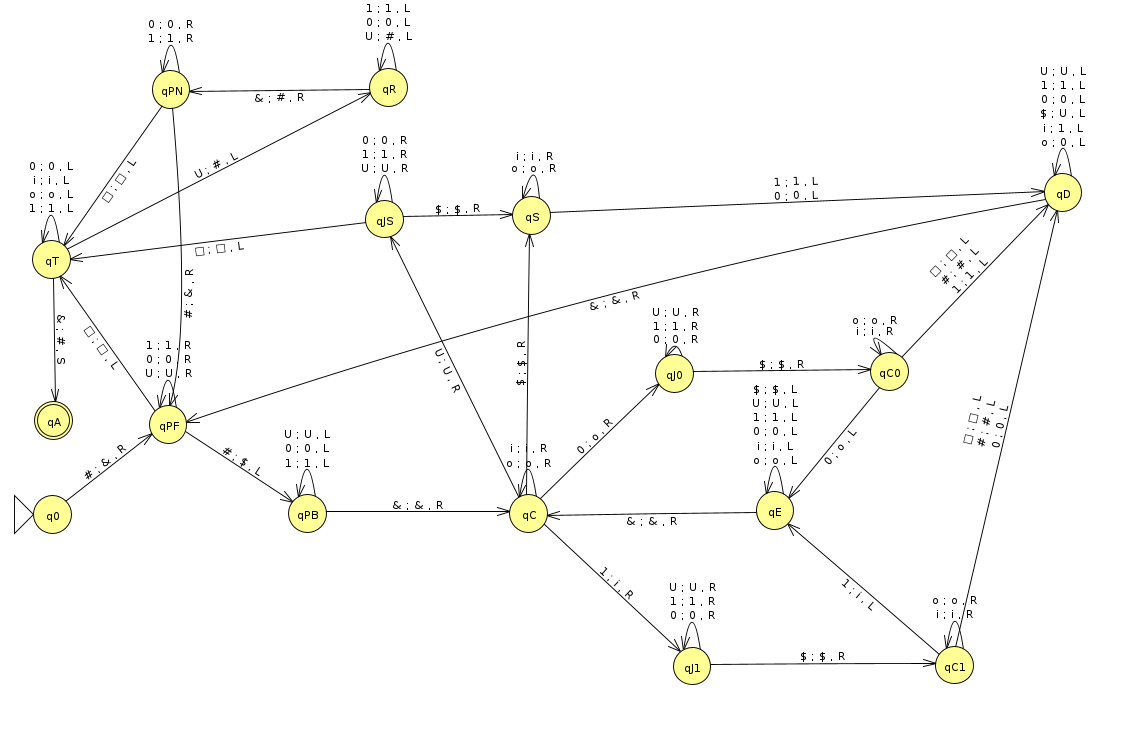
\includegraphics[width = 15 cm]{figs/M4Unicinta.png}
            \\
            \\
            Debido a la complejidad del diagrama, se puede ver su funcionamiento de manera más efectiva a través del simulador del siguiente enlace: \url{http://turingmachinesimulator.com/shared/oxlgudyvgv}
            \\
            \\
            Al igual que con la versión multicinta, todo el material necesario se encuentra disponible en el repositorio de \textit{GitHub}: \url{https://github.com/juanmagdev/AyC-Grupo-A1-04}
        \end{solution}
    \end{parts}

\end{questions}



%\hrule
%\subsection*{For retting}
%Ikke skriv noe her. \par \noindent
%\gradetable[h][questions]	
\end{document}